\documentclass{scrartcl}
\usepackage[utf8]{inputenc}
\usepackage{graphicx}
\title{Project: Power Cloud}
\subtitle{Client: Hanrich Potgieter \\\\\\\ Team: Quadcore Productions\\}
\author{Themba Mbhele 14007950\\ Moses Mayimela 14019702 \\ Hlengekile Jita 14077893 \\ Mpho Baloyi 14133670 \\Department of Computer Science, University of Pretoria}
\date{01 May 2016}


\begin{document}

\maketitle
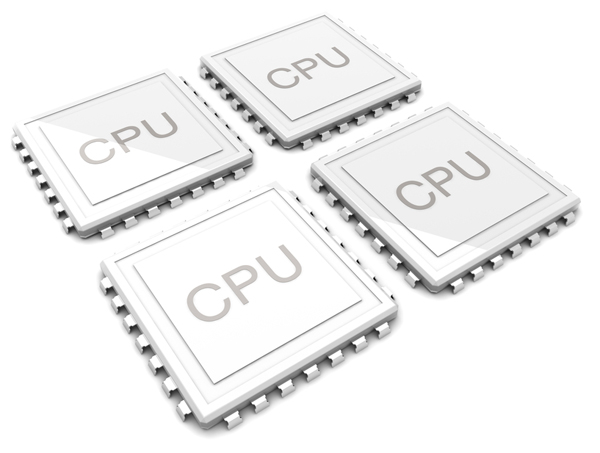
\includegraphics[width=\textwidth]{2012-quad-core-phones}
\section{The Team}
\subsection{Moses Mayimela}
\subsection{Hlengekile Jita}
\subsection{Mpho Baloyi}
\subsection{Themba Mbhele}

\section{Project Execution}
\subsection{Development Methodology}
\subsection{Communication With Client}
\subsection{Technical Challenges}
\subsection{Technologies}
This section will list the technologies that will be used to implement the system.\\
To implement the back-end of the system, the following technologies will be used:
\begin{itemize}
    \item NodeJS will be used to implement the server.
    \item MongoDB will be used to store the data that will be collected.
    \item C++ will be used to program the hardware
\end{itemize}
To implement the front-end of the system, the following technologies will be used:
\begin{itemize}
    \item AngularJS will be used for the web front-end.
\end{itemize}

\end{document}
